\documentclass[11pt,border=5pt]{standalone}
\usepackage{fontspec}
\setmainfont{cmunrm.otf}[BoldFont=cmunbx.otf,ItalicFont=cmunti.otf,BoldItalicFont=cmunbi.otf]
\usepackage{amsmath}
\usepackage{unicode-math}
\setmathfont{NewCMMath-Regular.otf}
\usepackage{tikz}
\usetikzlibrary{arrows.meta,patterns,angles,quotes}
\begin{document}
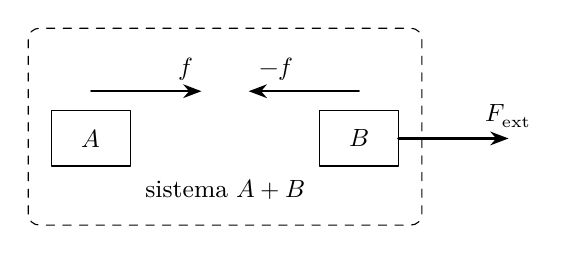
\begin{tikzpicture}[>=Stealth,font=\small,line cap=round,line join=round]
\draw[fill=white] (-2.2,-0.35) rectangle (-1.2,0.35);
\node at (-1.7,0) {$A$};
\draw[fill=white] (1.2,-0.35) rectangle (2.2,0.35);
\node at (1.7,0) {$B$};
\draw[dashed,rounded corners](-2.5,-1.1)rectangle(2.5,1.4);\draw[->,thick] (-1.7,0.6) -- (-0.3,0.6) node[above left] {$f$};
\draw[->,thick] (1.7,0.6) -- (0.3,0.6) node[above right] {$-f$};
\draw[->,thick] (2.2,0) -- (3.6,0) node[above] {$F_{\rm ext}$};
\node at (0,-0.65) {sistema $A+B$};

\end{tikzpicture}
\end{document}
